\documentclass[../main.tex]{subfiles}


\begin{document}
    Bezpieczne protokoły mogą być wykorzystywane:
    \begin{itemize}
        \item w warstwie aplikacji- szyfrowanie komunikatów HTTPS, protokoły SSL, TLS,
        \item między warstwą sieci a transportu- szyfrowanie
        pakietów IP – protokół IPSec,
        \item w warstwie łącza danych - szyfrowanie ramek, np. WEP,
        WPA, WPA2 w sieciach bezprzewodowych.
    \end{itemize}


    \subsection{Protokół IPSec}
    \begin{itemize}
        \item warstwa IP
        \item może szyfrować dane pochodzące z dowolnej
        aplikacji, proces szyfrowania i deszyfrowania jest niewidoczny dla użytkownika
        \item framework umożliwiający wykorzystanie pewnych protokołów (Authentication Headers AH i Encapsulating Security Payloads ESP)i
        metod według określonych zasad.
        \item \textbf{Authentication Headers} -  sprawdzenie autentyczności i integralności danych.\\
        \item \textbf{Encapsulating Security Payloads} - szyfrowanie danych, oraz autentyczność i integralność danych. ESP może być
        używany samodzielnie lub z AH.
    \end{itemize}

    Przed przesyłaniem danych strony komunikujące się uzgadniają szczegóły takie jak sposób
    uwierzytelniania, wymiana kluczy, algorytmy szyfrowania.

    Tryby działania IPSec (zarówno AH jak i ESP):
    \begin{itemize}
        \item Tryb transportu (w sieci lokalnej) między dwoma punktami końcowymi transmisji.
        \item Tryb tunelowania – szyfrowanie w niezabezpieczonej części sieci (np. dane między
        biurami przesyłane przez Internet).
    \end{itemize}

    Metody uwierzytelniania w IPSec:
    \begin{itemize}
        \item Kerberos,
        \item Oparty o certyfikaty cyfrowe,
        \item Klucz dzielony (przechowywany we właściwościach napis jednakowy dla obu
        komunikujących się stron).
    \end{itemize}

    \textbf{Filtry IPSec}\\
    Filtr IPSec pozwala na automatyczne przepuszczenie datagramów IP, blokowanie lub użycie
    negocjacji (i w konsekwencji użycie IPSec) w zależności od źródła i miejsca docelowego IP,
    protokołu transportowego, portów źródłowych i docelowych.


    \subsubsection{SSL - Secure Socket Layer}
    \begin{itemize}
        \item jego zadaniem jest zabezpieczanie informacji przesyłanych siecią.
        \item wykorzystywany przy przesyłaniu np. danych osobistych, numerów kart kredytowych.
        \item często prezentowany jako protokół, który leży
        powyżej warstwy transportu (TCP, UDP) i sieci (IP) a poniżej warstwy aplikacji (np. HTTP, FTP,
        SMTP, TELNET)
        \item W modelu ISO OSI jest przypisany do warstwy prezentacji (zatem do
        warstwy aplikacji w modelu TCP/IP)
        \item jest protokołem otwartym
        \item wykorzystuje szyfrowanie symetryczne z kluczem publicznym
        \item protokoły zabezpieczone SSL oznaczane są jako HTTPS (dla HTTP), FTPS (dla FTP) itd.
    \end{itemize}

    \begin{figure}[H]
        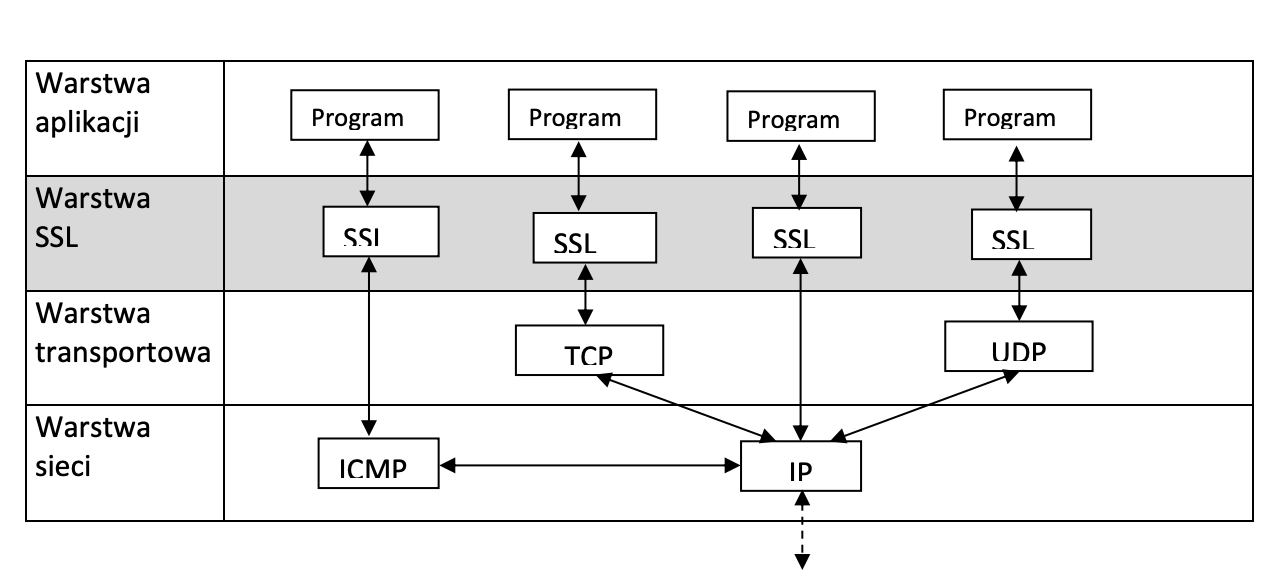
\includegraphics[width=\linewidth]{ssl.png}
    \end{figure}

    Podstawowe cechy protokołu SSL:
    \begin{itemize}
        \item Warstwa aplikacji.
        \item Zapewnia autoryzację serwerów internetowych i (opcjonalnie) klientów (utrudnia
        podszywanie pod autoryzowanych usługodawców i użytkowników)
        \item Zapewnia szyfrowanie - poufność przesyłanych informacji.
        \item Stosuje sumy kontrolne dla zapewnienia integralności danych.
    \end{itemize}

    Po nawiązaniu połączenia następuje wymiana informacji (certyfikatów CA i kluczy publicznych)
    uwierzytelniających serwera i (opcjonalnie) klienta.
    Serwer i klient uzgadniają również algorytmy szyfrowania –
    najsilniejsze dostępne jednocześnie obu stronom.
    Następnie serwer i klient generują klucze sesji (symetryczne), które są szyfrowane kluczem
    publicznym drugiej strony. Klucze sesji są odszyfrowywane przy pomocy klucza prywatnego i
    następnie służą do szyfrowania danych.

    \subsection{TLS - Transport Layer Security}
    \begin{itemize}
        \item warstwa aplikacji
        \item strony dogadują się co do klucza symetrycznego szyfrowaniem niesymetrycznym
        \item przy danych nie ma asymetrycznego szyfrowania, tylko symetryczne
    \end{itemize}

\end{document}